\documentclass[conference]{IEEEtran}

\usepackage{cite}
\usepackage{amsmath,amssymb,amsfonts}
\usepackage{graphicx}
\usepackage{textcomp}
\usepackage{xcolor}
\usepackage{booktabs}
\usepackage{float}
\usepackage{url}
\usepackage{multirow}
\usepackage{array}

% Pull figures from the project images/ folder; fall back to the local folder.
\graphicspath{{../images/}{./}}

\begin{document}

\title{NBA Free Throw Prediction Using Machine Learning Classification Models}

\author{

\IEEEauthorblockN{
Habibatallah Mahdi,
Sama Abdelsadek,
Mohamed Allam,
Shaza Hossam,
Ahmed Shaban
}

\IEEEauthorblockA{
Department of Computer Science \\
School of Information Technology and Computer Science \\
Nile University \\
El Sheikh Zayed, Giza, Egypt
}

}

\maketitle

% =========================================================
% ABSTRACT
% =========================================================

\begin{abstract}

Free-throw shooting is a decisive, high-frequency skill in basketball, yet it is only partially explained by the rest of a player's box-score profile. This project presents a machine learning system that classifies an NBA player-season as a \textit{good} free-throw shooter (free-throw percentage at or above 75\%) or a \textit{below-average} free-throw shooter (below 75\%) using season-long statistics. A dataset of 26{,}292 player-season records covering the 1975--2025 NBA seasons was collected by web scraping Basketball Reference and was augmented with scraped player height and weight from a second source. After removing traded-player duplicates and keeping only player-seasons with a meaningful free-throw sample, 15{,}020 records described by 39 features remained. Particular care was taken to avoid data leakage: free throws made, free-throw attempts, and free-throw percentage are excluded from the feature set because they directly determine the target label. Five classification algorithms --- K-Nearest Neighbors, Support Vector Classifier, Logistic Regression, Random Forest, and Gradient Boosting --- were trained with default-configuration estimators and compared using accuracy, precision, recall, F1-score, and confusion matrices. Gradient Boosting achieved the highest test accuracy of 78.06\%. The system is deployed as an interactive Streamlit web application that generates real-time predictions for user-supplied player profiles.

\end{abstract}

\begin{IEEEkeywords}
Machine Learning, Sports Analytics, NBA, Classification, Free Throw Prediction, Data Leakage, Web Scraping
\end{IEEEkeywords}

% =========================================================
% INTRODUCTION
% =========================================================

\section{Introduction}

Machine learning has become one of the most influential technologies in sports analytics. Basketball organizations increasingly use data-driven systems to evaluate players, optimize team strategies, and support recruitment and rotation decisions. Among individual skills, free-throw shooting stands out: free throws are uncontested, occur in large volume, and frequently decide the outcome of close games during clutch moments.

Free-throw efficiency is, however, a specific physical and mental skill that is only partially correlated with the rest of a player's statistical profile. A high-scoring guard and a low-usage center may share many box-score similarities yet differ sharply at the free-throw line. This makes free-throw classification a genuinely non-trivial learning problem rather than a simple statistical lookup.

This project builds a machine learning classification system that predicts whether an NBA player-season is a good or a below-average free-throw shooter, using season-long box-score statistics together with engineered and historical features. The project is organized into two phases:

\begin{itemize}
\item \textbf{Phase 1:} Problem definition, data collection, preprocessing, feature engineering, and initial model training.
\item \textbf{Phase 2:} Systematic model evaluation and comparison, result visualization, deployment as an interactive web application, and preparation of this final paper.
\end{itemize}

The main contributions of the work are: (1) an original dataset assembled by web scraping two distinct Basketball Reference sources and integrating them; (2) a preprocessing pipeline that explicitly prevents data leakage, which is the single most common cause of misleadingly optimistic results in this type of task; (3) a fair comparison of five classification algorithms trained with default-configuration estimators; and (4) a deployed Streamlit dashboard that makes the trained models usable in real time.

% =========================================================
% PROBLEM STATEMENT
% =========================================================

\section{Problem Statement}

The objective of this project is to classify each NBA player-season into one of two categories based on free-throw percentage (FT\%):

\begin{itemize}
\item \textbf{Good free-throw shooter} --- FT\% $\geq$ 0.75
\item \textbf{Below-average free-throw shooter} --- FT\% $<$ 0.75
\end{itemize}

The task is therefore a supervised binary classification problem. The challenge is to learn this distinction \textit{without} access to any free-throw quantity for the season being predicted, relying instead on the player's other statistics, physical attributes, engineered ratios, and free-throw record from \textit{previous} seasons.

A correctly designed system of this type can support coaches, analysts, scouts, and front-office staff by flagging players who are likely to be reliable or unreliable at the line, informing rotation choices, late-game lineups, and contract evaluation.

% =========================================================
% DATASET
% =========================================================

\section{Dataset Description}

\subsection{Data Source}

In accordance with the course requirement that datasets be self-collected from reputable sources rather than downloaded ready-made, the dataset was assembled by web scraping Basketball Reference using Python with the \texttt{requests}, \texttt{BeautifulSoup}, and \texttt{lxml} libraries. Two distinct sources were scraped and merged:

\begin{itemize}
\item Per-game player statistics for every NBA season from 1975 to 2025, from the per-game season leaderboards.\footnote{\url{https://www.basketball-reference.com/leagues/}}
\item Player biographical data (height and weight) from the Basketball Reference player index pages.\footnote{\url{https://www.basketball-reference.com}}
\end{itemize}

Combining these two sources is the data-integration element of the project: the height and weight attributes do not exist in the per-game tables and had to be scraped separately and joined on the player name.

\subsection{Dataset Overview}

\begin{table}[H]
\centering
\caption{Dataset Overview}
\begin{tabular}{|l|l|}
\hline
\textbf{Property} & \textbf{Value} \\
\hline
Primary source & Basketball Reference \\
\hline
Secondary source & Basketball Reference player index \\
\hline
Timeframe & 1975 -- 2025 \\
\hline
Raw rows & 26,292 \\
\hline
Raw columns & 32 \\
\hline
Modeling rows & 15,020 \\
\hline
Modeling features & 39 \\
\hline
Task type & Binary classification \\
\hline
\end{tabular}
\label{tab:dataset}
\end{table}

The raw per-game table contains standard season-average statistics, including Games Played (G), Games Started (GS), Minutes Played (MP), field-goal counts and percentages (FG, FGA, FG\%), three-point counts and percentages (3P, 3PA, 3P\%), two-point counts and percentages (2P, 2PA, 2P\%), effective field-goal percentage (eFG\%), offensive, defensive and total rebounds (ORB, DRB, TRB), assists (AST), steals (STL), blocks (BLK), turnovers (TOV), personal fouls (PF), and points per game (PTS). Free-throw columns (FT, FTA, FT\%) are present in the raw data but are deliberately excluded from the feature set, as explained in Section~\ref{sec:leakage}.

% =========================================================
% PROJECT WORKFLOW
% =========================================================

\section{Project Workflow}

The project followed a structured machine learning pipeline:

\begin{enumerate}
\item Web scraping of NBA per-game statistics and player biographical data.
\item Data cleaning and preprocessing.
\item Target label construction.
\item Feature engineering and integration of the external bio data.
\item Feature scaling for distance- and margin-based models.
\item Model training with default-configuration estimators.
\item Model evaluation and comparison across five algorithms.
\item Deployment of an interactive Streamlit web application.
\end{enumerate}

% =========================================================
% PREPROCESSING
% =========================================================

\section{Data Preprocessing}

Preprocessing was performed in a dedicated notebook and is fully reproducible. Table~\ref{tab:funnel} summarizes how the row count evolves through the cleaning pipeline.

\begin{table}[H]
\centering
\caption{Row Count Through the Preprocessing Pipeline}
\begin{tabular}{|l|c|}
\hline
\textbf{Stage} & \textbf{Rows} \\
\hline
Raw scraped data & 26,292 \\
\hline
After dropping unused columns & 26,292 \\
\hline
After traded-player de-duplication & 21,276 \\
\hline
After removing invalid position rows & 21,275 \\
\hline
After free-throw sample filter (FTA $\geq$ 1) & 15,020 \\
\hline
\end{tabular}
\label{tab:funnel}
\end{table}

\subsection{Handling Missing Values and Unused Columns}

The \texttt{Awards} column was empty for more than 23{,}000 of the 26{,}292 rows and was dropped entirely. The \texttt{Rk} column is only a display row index and was also dropped. Early seasons (1975--1979) predate the three-point line, so 3P, 3PA, and 3P\% are missing for those players; these were filled with 0, which is the correct value because those players genuinely attempted no three-pointers. Games Started (GS) is unrecorded before 1982 and was likewise filled with 0. After these steps the dataset contained no missing values.

\subsection{Duplicate Player-Season Handling}

When a player is traded mid-season, Basketball Reference lists one row per team plus a combined total row (labeled \texttt{TOT}, \texttt{2TM}, or \texttt{3TM}). For each (season, player) pair, only the combined row was kept, so each player-season is represented exactly once. This reduced the data from 26{,}292 to 21{,}276 rows. A single row with an invalid position label was then removed.

\subsection{Free-Throw Sample Filter}

Only player-seasons with at least one free-throw attempt per game (FTA $\geq$ 1.0) were retained. Players with very few attempts have an unstable FT\% --- a player who takes two free throws all season and makes both has a FT\% of 100\%, which is not a meaningful measure of skill. This filter ensures every retained row has a stable, interpretable free-throw percentage and left 15{,}020 modeling rows.

\subsection{Target Label Construction}

The target is a binary label defined by a fixed threshold on season free-throw percentage:

\begin{equation}
\text{Target} =
\begin{cases}
1, & \text{if FT\%} \geq 0.75 \quad (\text{Good}) \\
0, & \text{if FT\%} < 0.75 \quad (\text{Below-Average})
\end{cases}
\end{equation}

The value 0.75 was chosen deliberately for four reasons:

\begin{itemize}
\item It is the universally recognized NBA free-throw benchmark and is therefore immediately interpretable to any reader or analyst.
\item It is defined \textit{independently of the dataset}. A threshold based on the league-average FT\% would make every row's label depend on aggregate statistics of other rows; a fixed constant does not, which is methodologically cleaner.
\item It is effectively era-independent. The NBA league-average FT\% moved only between 0.728 and 0.784 across all 50 seasons studied; measured label agreement between a fixed-0.75 target and a per-season league-average target is 94.8\%, so the two definitions are nearly equivalent and the simpler one is preferred.
\item The median FT\% of the filtered data is 0.758, so the 0.75 threshold produces a well-balanced split.
\end{itemize}

After labeling, the dataset contains 8{,}151 good shooters (54.3\%) and 6{,}869 below-average shooters (45.7\%), shown in Fig.~\ref{fig:balance}. This near-balanced distribution reduces classification bias and makes accuracy a meaningful headline metric without resampling.

\begin{figure}[H]
\centering
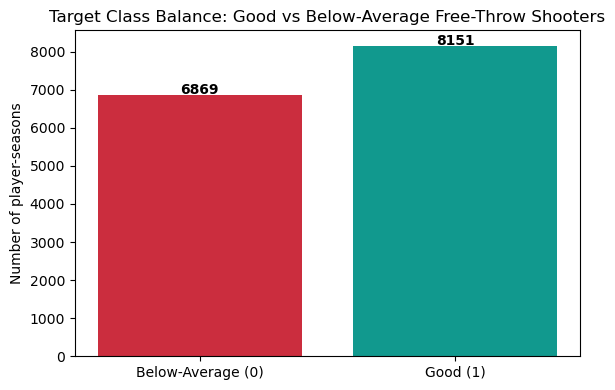
\includegraphics[width=0.42\textwidth]{eda_target_balance.png}
\caption{Target class balance: good versus below-average free-throw shooters.}
\label{fig:balance}
\end{figure}

\subsection{Data Leakage Prevention}
\label{sec:leakage}

The single most important design decision in this project is the explicit prevention of \textit{data leakage}. The columns FT (free throws made), FTA (free-throw attempts), and FT\% (free-throw percentage) are \textbf{never} used as model features:

\begin{itemize}
\item FT\% is the direct source of the target label.
\item FT and FTA together allow FT\% to be reconstructed exactly, since FT\% $=$ FT $/$ FTA.
\end{itemize}

Including any of these would let a model re-derive the target from its own definition, producing an artificially high accuracy that would not generalize to genuine prediction. These columns are dropped from the feature set in the preprocessing notebook.

\subsection{Historical Free-Throw Features}

Although the current season's free-throw statistics are excluded, a player's free-throw record from \textit{prior} seasons is both legitimate and highly informative. Three historical features were engineered using only data observed before the season being predicted:

\begin{itemize}
\item \texttt{career\_ft\_pct}: cumulative FT\% over all of the player's previous seasons.
\item \texttt{prev\_ft\_pct}: FT\% in the immediately preceding season.
\item \texttt{career\_seasons}: number of prior seasons played (0 for a rookie).
\end{itemize}

These are computed with chronologically ordered cumulative operations that exclude the current row, so no future information leaks backward. For rookie seasons, where no history exists, \texttt{career\_ft\_pct} and \texttt{prev\_ft\_pct} were filled with the global mean FT\% of 0.7414, a neutral prior for an unobserved player.

\subsection{Integration of External Bio Data}

Player height and weight, scraped separately, were merged into the dataset on player name, successfully matching 14{,}530 of the 15{,}020 player-seasons. The small number of unmatched rows were filled with the median height and weight. These two attributes (\texttt{height\_in}, \texttt{weight\_lb}) constitute the multi-source integration component of the project.

\subsection{Feature Engineering}

Six ratio features were engineered to capture playing style and efficiency beyond raw counting statistics:

\begin{itemize}
\item \texttt{ast\_to\_tov} $=$ AST $/$ TOV --- ball-handling efficiency.
\item \texttt{pts\_per\_fga} $=$ PTS $/$ FGA --- scoring efficiency per shot.
\item \texttt{threep\_rate} $=$ 3PA $/$ FGA --- reliance on three-point shooting.
\item \texttt{reb\_per\_min} $=$ TRB $/$ MP --- rebounding intensity.
\item \texttt{stocks\_per\_min} $=$ (STL $+$ BLK) $/$ MP --- defensive activity.
\item \texttt{scoring\_load} $=$ FGA $/$ MP --- shooting volume per minute.
\end{itemize}

Division by zero was handled by treating a zero denominator as a ratio of zero. The categorical \texttt{Pos} field was reduced to a primary position and one-hot encoded into five indicator columns (\texttt{Pos\_C}, \texttt{Pos\_PF}, \texttt{Pos\_PG}, \texttt{Pos\_SF}, \texttt{Pos\_SG}). The final modeling matrix contains 39 features, listed by group in Table~\ref{tab:features}.

\begin{table}[H]
\centering
\caption{Feature Groups (39 Features Total)}
\begin{tabular}{|l|p{5.2cm}|}
\hline
\textbf{Group} & \textbf{Features} \\
\hline
Playing time & Age, G, GS, MP \\
\hline
Shooting & FG, FGA, FG\%, 3P, 3PA, 3P\%, 2P, 2PA, 2P\%, eFG\% \\
\hline
Counting stats & ORB, DRB, TRB, AST, STL, BLK, TOV, PF, PTS \\
\hline
Historical FT & career\_ft\_pct, prev\_ft\_pct, career\_seasons \\
\hline
Physical (bio) & height\_in, weight\_lb \\
\hline
Engineered ratios & ast\_to\_tov, pts\_per\_fga, threep\_rate, reb\_per\_min, stocks\_per\_min, scoring\_load \\
\hline
Position (one-hot) & Pos\_C, Pos\_PF, Pos\_PG, Pos\_SF, Pos\_SG \\
\hline
\end{tabular}
\label{tab:features}
\end{table}

\subsection{Train-Test Split}

The dataset was divided into 80\% training data (12{,}016 rows) and 20\% test data (3{,}004 rows) using a fixed random seed (\texttt{random\_state = 42}). The identical split is reproduced in every model notebook and in the comparison notebook, so all five algorithms are trained and evaluated on exactly the same data.

\subsection{Feature Scaling}

Feature scaling was applied with \texttt{StandardScaler} for the three models sensitive to feature magnitude --- KNN, SVC, and Logistic Regression --- while the tree-based models (Random Forest and Gradient Boosting) were trained on raw, unscaled features, as tree splits are invariant to monotonic feature transformations. To avoid leakage from the test set, each scaler was fit on the training set only and then applied to the test set. The standardization transform is:

\begin{equation}
Z = \frac{X - \mu}{\sigma}
\end{equation}

where $X$ is the original value, $\mu$ the training-set mean, and $\sigma$ the training-set standard deviation. All preprocessing steps were implemented procedurally, without scikit-learn \texttt{Pipeline} objects, so that every transformation is explicit and inspectable.

\begin{figure}[H]
\centering
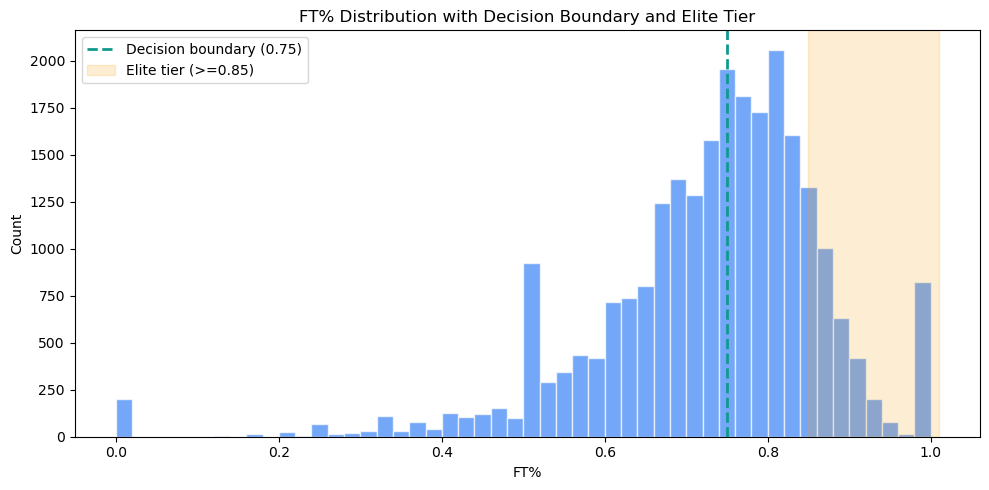
\includegraphics[width=0.46\textwidth]{eda_ft_distribution.png}
\caption{Distribution of season FT\% across all players. The dashed line marks the 0.75 decision boundary; the shaded region marks the elite tier (FT\% $\geq$ 0.85).}
\label{fig:ftdist}
\end{figure}

% =========================================================
% EXPLORATORY DATA ANALYSIS
% =========================================================

\section{Exploratory Data Analysis}

Exploratory analysis was carried out before modeling to understand the data and to guide feature engineering.

Fig.~\ref{fig:ftdist} shows the distribution of season FT\%. The bulk of player-seasons lie between 0.60 and 0.85, with the 0.75 decision boundary cutting through the dense central region --- confirming that the chosen threshold separates a genuinely contested population rather than trivially splitting clear extremes.

Fig.~\ref{fig:corr} ranks every numeric feature by its Pearson correlation with the target. The strongest \textit{positive} predictors are three-point activity (3PA, 3P, \texttt{threep\_rate}, 3P\%), overall scoring (PTS, FGA), and the historical free-throw features (\texttt{prev\_ft\_pct}, \texttt{career\_ft\_pct}). The strongest \textit{negative} predictors are interior-play indicators: \texttt{reb\_per\_min}, height, weight, blocks, and offensive rebounds. This matches basketball intuition --- perimeter shooters tend to be reliable free-throw shooters, while big men generally are not.

Fig.~\ref{fig:league} plots the NBA league-average FT\% over time. It stays within the narrow 0.728--0.784 band across five decades, which empirically justifies treating the fixed 0.75 threshold as era-independent.

\begin{figure}[H]
\centering
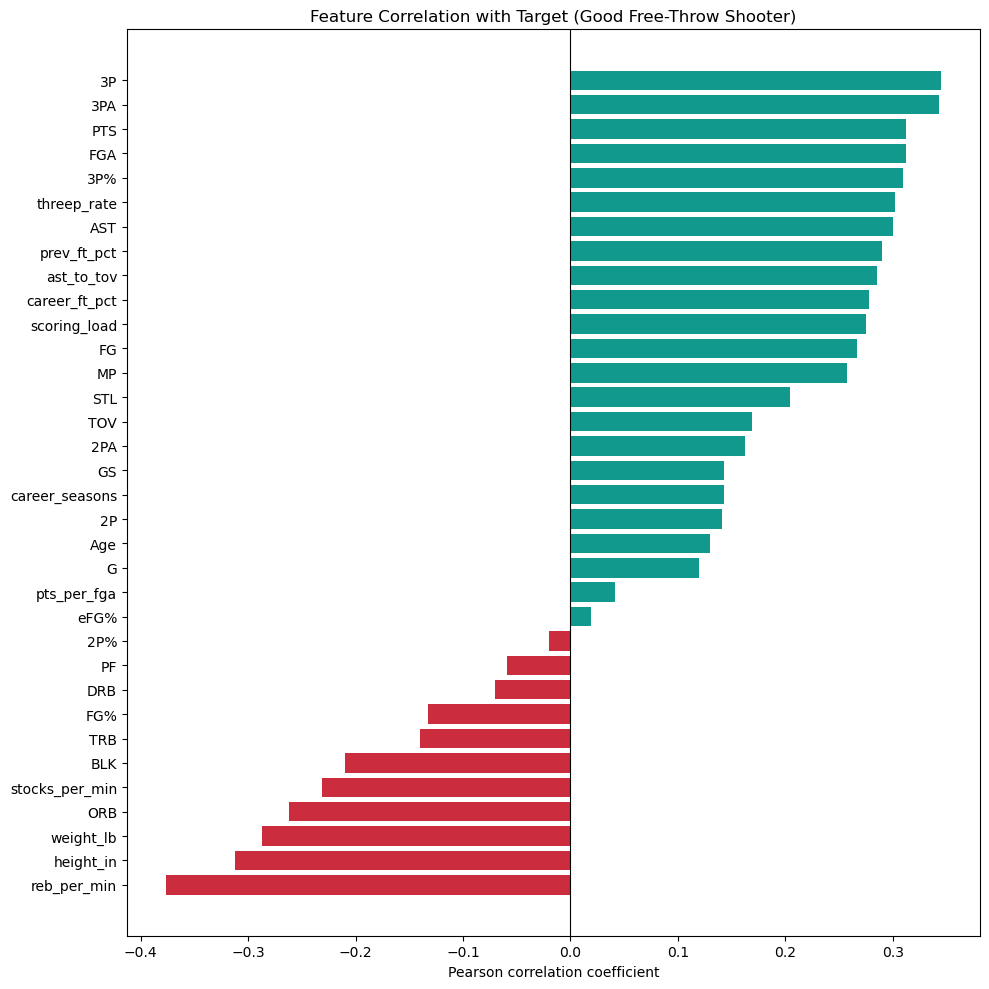
\includegraphics[width=0.44\textwidth]{eda_feature_correlation.png}
\caption{Pearson correlation of each feature with the target. Green bars are positive predictors, red bars negative.}
\label{fig:corr}
\end{figure}

\begin{figure}[H]
\centering
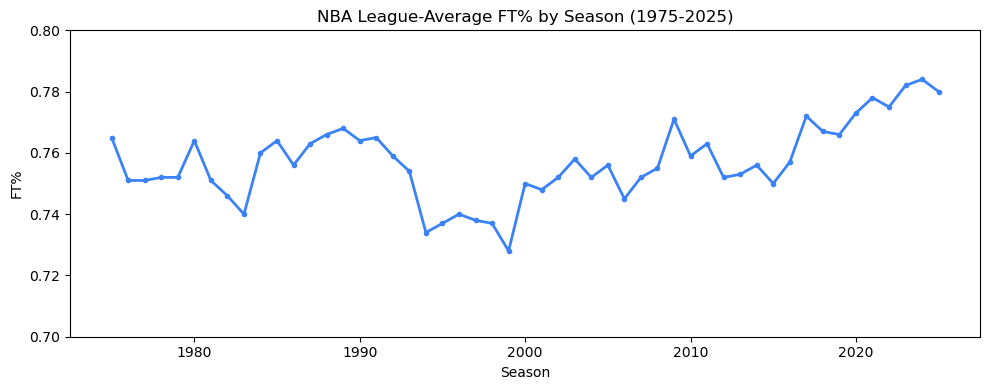
\includegraphics[width=0.46\textwidth]{eda_league_avg_ft.png}
\caption{NBA league-average FT\% by season (1975--2025). The value stays within a narrow band, supporting an era-independent fixed threshold.}
\label{fig:league}
\end{figure}

% =========================================================
% MODELS
% =========================================================

\section{Machine Learning Models}

Five classification algorithms were implemented, one as the primary responsibility of each team member, all on the identical dataset and train-test split. Each model was trained with its default configuration using fixed constructor settings. Table~\ref{tab:hyper} lists the configuration used for each model.

\subsection{K-Nearest Neighbors}

KNN classifies a player-season by majority vote among its $k$ most similar training examples in the standardized feature space. It is non-parametric and makes no assumption about the form of the decision boundary, but it is sensitive to feature scaling and to the dimensionality of the space. The model uses $k = 5$ neighbors.

\subsection{Support Vector Classifier}

SVC finds the decision boundary that maximizes the margin between the two classes. An RBF kernel is used so that the model can represent non-linear boundaries, with default scikit-learn regularization and gamma settings.

\subsection{Logistic Regression}

Logistic Regression models the log-odds of the positive class as a linear combination of the features. It is fast, stable, and highly interpretable, and serves as a strong linear baseline against the non-linear models. The model uses the \texttt{liblinear} solver with a maximum of 1{,}000 iterations.

\subsection{Random Forest}

Random Forest trains many decision trees on bootstrapped samples with random feature subsets and averages their votes. This reduces the variance of individual trees and captures non-linear feature interactions. The model uses 100 trees with default depth settings.

\subsection{Gradient Boosting}

Gradient Boosting builds an ensemble of shallow decision trees sequentially, where each new tree corrects the errors of the current ensemble. The model uses 100 estimators, a learning rate of 0.1, and a maximum depth of 3.

\begin{table}[H]
\centering
\caption{Model Configurations}
\begin{tabular}{|l|p{5.0cm}|}
\hline
\textbf{Model} & \textbf{Key constructor arguments} \\
\hline
KNN & n\_neighbors $= 5$ \\
\hline
SVC & kernel $=$ rbf; default C and gamma \\
\hline
Logistic Regression & solver $=$ liblinear; max\_iter $= 1000$ \\
\hline
Random Forest & n\_estimators $= 100$; random\_state $= 42$ \\
\hline
Gradient Boosting & n\_estimators $= 100$; learning\_rate $= 0.1$; max\_depth $= 3$; random\_state $= 42$ \\
\hline
\end{tabular}
\label{tab:hyper}
\end{table}

% =========================================================
% MODEL EVALUATION
% =========================================================

\section{Evaluation Metrics}

Because the two classes are nearly balanced, accuracy is a meaningful headline metric, but it is reported together with precision, recall, F1-score, and the confusion matrix to give a complete picture of each model's behavior. The metrics are defined as:

\begin{equation}
\text{Accuracy} = \frac{TP + TN}{TP + TN + FP + FN}
\end{equation}

\begin{equation}
\text{Precision} = \frac{TP}{TP + FP}
\end{equation}

\begin{equation}
\text{Recall} = \frac{TP}{TP + FN}
\end{equation}

\begin{equation}
\text{F1} = 2 \cdot \frac{\text{Precision} \cdot \text{Recall}}{\text{Precision} + \text{Recall}}
\end{equation}

where $TP$, $TN$, $FP$, and $FN$ are the counts of true positives, true negatives, false positives, and false negatives. Precision, recall, and F1 are reported for the positive class (good shooter). All evaluation uses the same held-out 20\% test set of 3{,}004 player-seasons.

% =========================================================
% RESULTS
% =========================================================

\section{Experimental Results}

Table~\ref{tab:results} reports the test-set performance of all five models, ordered by accuracy. Gradient Boosting achieved the best accuracy at 78.06\%, ahead of SVC at 77.23\% and Random Forest at 76.96\%. Logistic Regression and KNN trailed at 74.23\% and 71.64\% respectively. The accuracy comparison is visualized in Fig.~\ref{fig:comparison}.

\begin{table}[H]
\centering
\caption{Model Performance on the Test Set (\%)}
\begin{tabular}{|l|c|c|c|c|}
\hline
\textbf{Model} & \textbf{Accuracy} & \textbf{Precision} & \textbf{Recall} & \textbf{F1} \\
\hline
Gradient Boosting & \textbf{78.06} & 79.65 & 79.70 & 79.68 \\
\hline
SVC & 77.23 & 78.31 & 79.95 & 79.12 \\
\hline
Random Forest & 76.96 & 79.09 & 77.91 & 78.50 \\
\hline
Logistic Regression & 74.23 & 75.25 & 77.85 & 76.53 \\
\hline
KNN & 71.64 & 73.35 & 74.52 & 73.93 \\
\hline
\end{tabular}
\label{tab:results}
\end{table}

\begin{figure}[H]
\centering
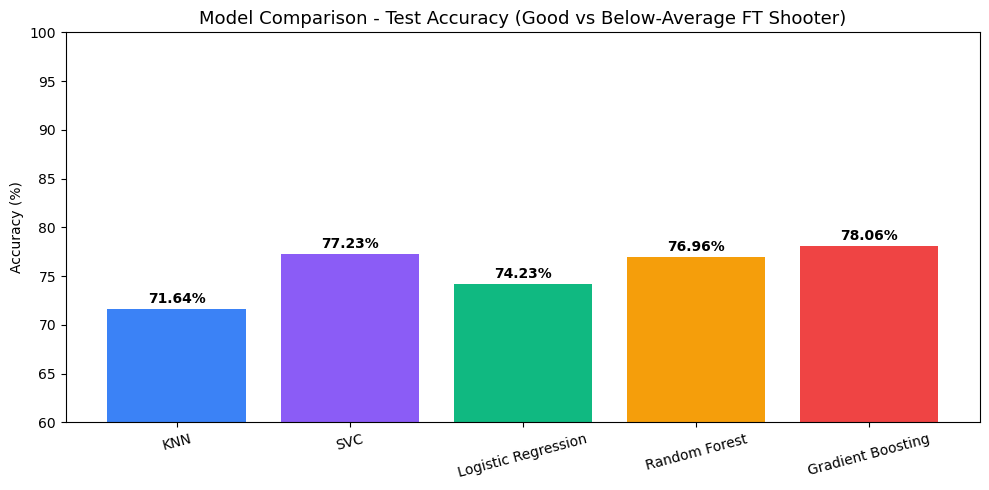
\includegraphics[width=0.48\textwidth]{model_comparison.png}
\caption{Test accuracy of the five classification models.}
\label{fig:comparison}
\end{figure}

The confusion matrices in Fig.~\ref{fig:cm_gb} through Fig.~\ref{fig:cm_knn} show how each model distributes its predictions across the two classes. The strongest models are roughly symmetric, making a similar number of errors on each class, which is desirable given the balanced target.

\begin{figure}[H]
\centering

\includegraphics[width=0.40\textwidth]{gb_confusion_matrix.png}
\caption{Gradient Boosting confusion matrix.}
\label{fig:cm_gb}
\end{figure}

\begin{figure}[H]
\centering
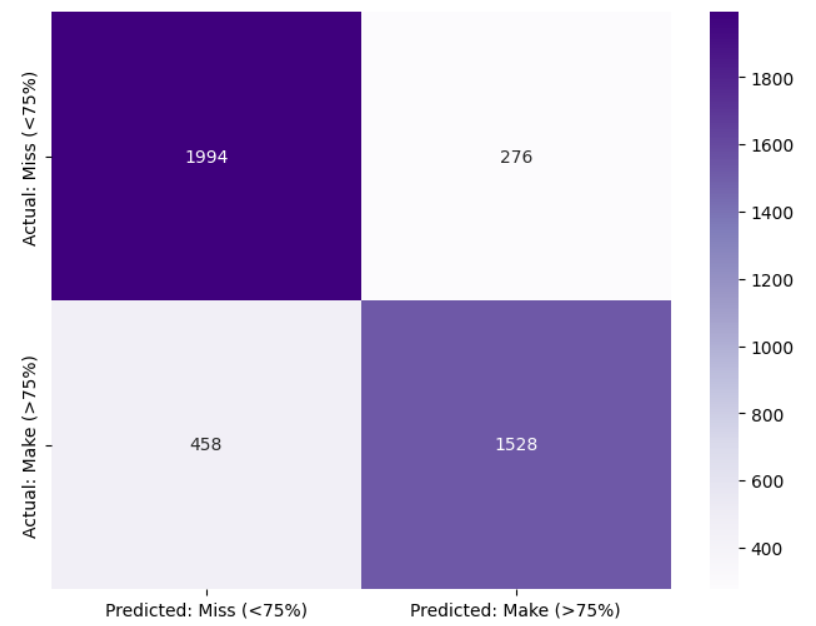
\includegraphics[width=0.40\textwidth]{svc_confusion_matrix.png}
\caption{SVC confusion matrix.}
\label{fig:cm_svc}
\end{figure}

\begin{figure}[H]
\centering
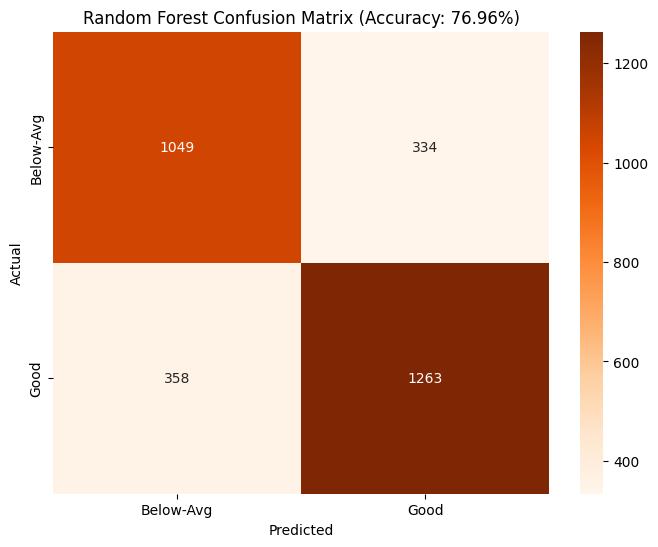
\includegraphics[width=0.40\textwidth]{rf_confusion_matrix.png}
\caption{Random Forest confusion matrix.}
\label{fig:cm_rf}
\end{figure}

\begin{figure}[H]
\centering
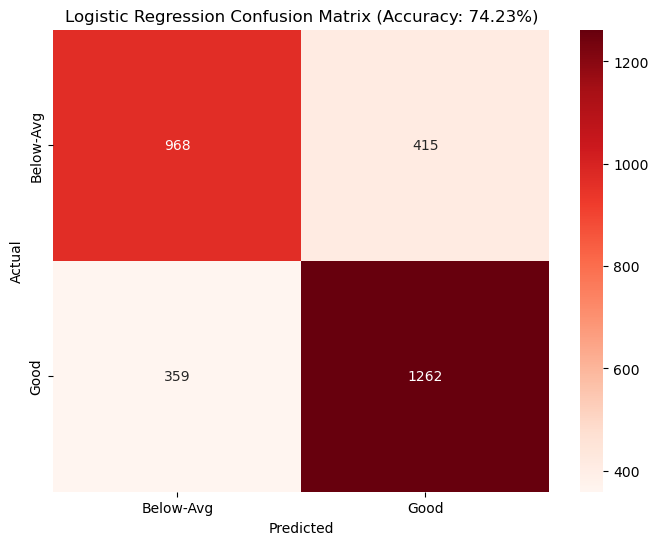
\includegraphics[width=0.40\textwidth]{lr_confusion_matrix.png}
\caption{Logistic Regression confusion matrix.}
\label{fig:cm_lr}
\end{figure}

\begin{figure}[H]
\centering
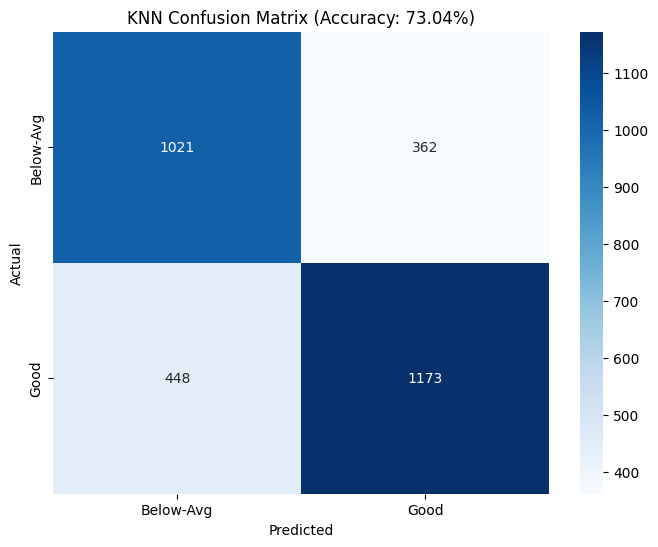
\includegraphics[width=0.40\textwidth]{knn_confusion_matrix.png}
\caption{KNN confusion matrix.}
\label{fig:cm_knn}
\end{figure}

% =========================================================
% DISCUSSION
% =========================================================

\section{Discussion}

\subsection{Why the Models Cluster in the 73--78\% Range}

All five models fall within a 71--78\% accuracy band. This is an honest and expected result rather than a weakness. Because the fixed 0.75 threshold classifies \textit{every} player-season that has a meaningful free-throw sample --- nobody is excluded --- the models must label the genuinely uncertain players who shoot close to 75\%. The 71--78\% range therefore reflects what machine learning can realistically achieve on the full population, including the hard middle cases, rather than an inflated figure obtained by only testing on clear extremes.

\subsection{Comparison and Trade-offs}

The non-linear models (Gradient Boosting, SVC, Random Forest) outperformed Logistic Regression, indicating that the relationship between box-score statistics and free-throw skill is not fully linearly separable. Gradient Boosting and SVC were essentially tied at the top; Gradient Boosting is preferable in deployment because it does not require feature scaling and exposes feature importances, while SVC is more sensitive to its hyperparameters and scales less well to larger data. Random Forest performed slightly below the other two ensembles but remains competitive and is the most robust to overfitting with minimal tuning.

KNN produced the weakest result. In a 39-dimensional feature space, distance-based neighbor voting suffers from the curse of dimensionality: distances become less discriminative, so even $k = 5$ neighbors cannot match the structured models. Logistic Regression, although linear, still produced a respectable 74.23\% and is the most interpretable model, making it a reasonable lightweight baseline.

In summary, there is a clear trade-off: Logistic Regression offers interpretability and speed, KNN offers conceptual simplicity but poor high-dimensional behavior, and the ensemble and kernel methods offer the best accuracy at the cost of interpretability and tuning effort.

\subsection{What Drives the Predictions}

The exploratory correlation analysis (Fig.~\ref{fig:corr}) and the model behavior agree: the historical free-throw features (\texttt{career\_ft\_pct}, \texttt{prev\_ft\_pct}) and perimeter-shooting features (3PA, 3P, \texttt{threep\_rate}) are the strongest signals. This is intuitive --- free-throw shooting is a stable individual skill, so a player's own past record is the best available evidence, and perimeter shooting and free-throw shooting share an underlying shooting touch.

\subsection{Role of the External Bio Data}

The height and weight features form the multi-source data-integration component of the project. Their measured contribution to predictive accuracy is marginal, because height and weight are already partially reflected in position and rebounding statistics. They were nonetheless retained, both because they are the project's genuine data-integration element and because reporting their limited impact honestly is itself a point of methodological rigor.

\subsection{Alternative Threshold Framing}

An alternative, stricter design would classify only \textit{elite} shooters (FT\% $\geq$ 0.85) against \textit{weak} shooters (FT\% $<$ 0.65), discarding the ambiguous middle group. That framing can reach a higher headline accuracy of roughly 92\%, but only because it removes the roughly 47\% of players who are hardest to classify --- the model is never asked to make a difficult call. The fixed 0.75 threshold was chosen as the primary target precisely because it classifies every player-season and therefore produces an honest estimate of real-world performance.

% =========================================================
% STREAMLIT
% =========================================================

\section{Phase 2: Streamlit Deployment}

To make the trained models usable in practice, the system was deployed as an interactive web application built with Streamlit. The application loads the five trained models, their scalers, and the saved ordered feature list, and provides three pages reachable from a sidebar menu:

\begin{itemize}
\item \textbf{Home} --- a project summary with key dataset statistics and the best-performing model.
\item \textbf{Prediction} --- an input form, organized into free-throw history, player information, shooting statistics, and performance groups, where the user enters statistics and selects a model.
\item \textbf{Model Comparison} --- the results table, the accuracy bar chart, and all five confusion matrices.
\end{itemize}

On the prediction page, the application reconstructs the full 39-feature vector from the user's inputs: it computes the engineered ratio features, derives the made-shot counts, one-hot encodes the position, and reindexes the row to the exact training feature order stored in \texttt{feature\_columns.pkl}. The appropriate scaler is then applied for KNN, SVC, and Logistic Regression, while Random Forest and Gradient Boosting receive the raw vector. The selected model returns a real-time classification of the player as a good or below-average free-throw shooter. Fig.~\ref{fig:home} and Fig.~\ref{fig:prediction} show the interface.

\begin{figure}[H]
\centering
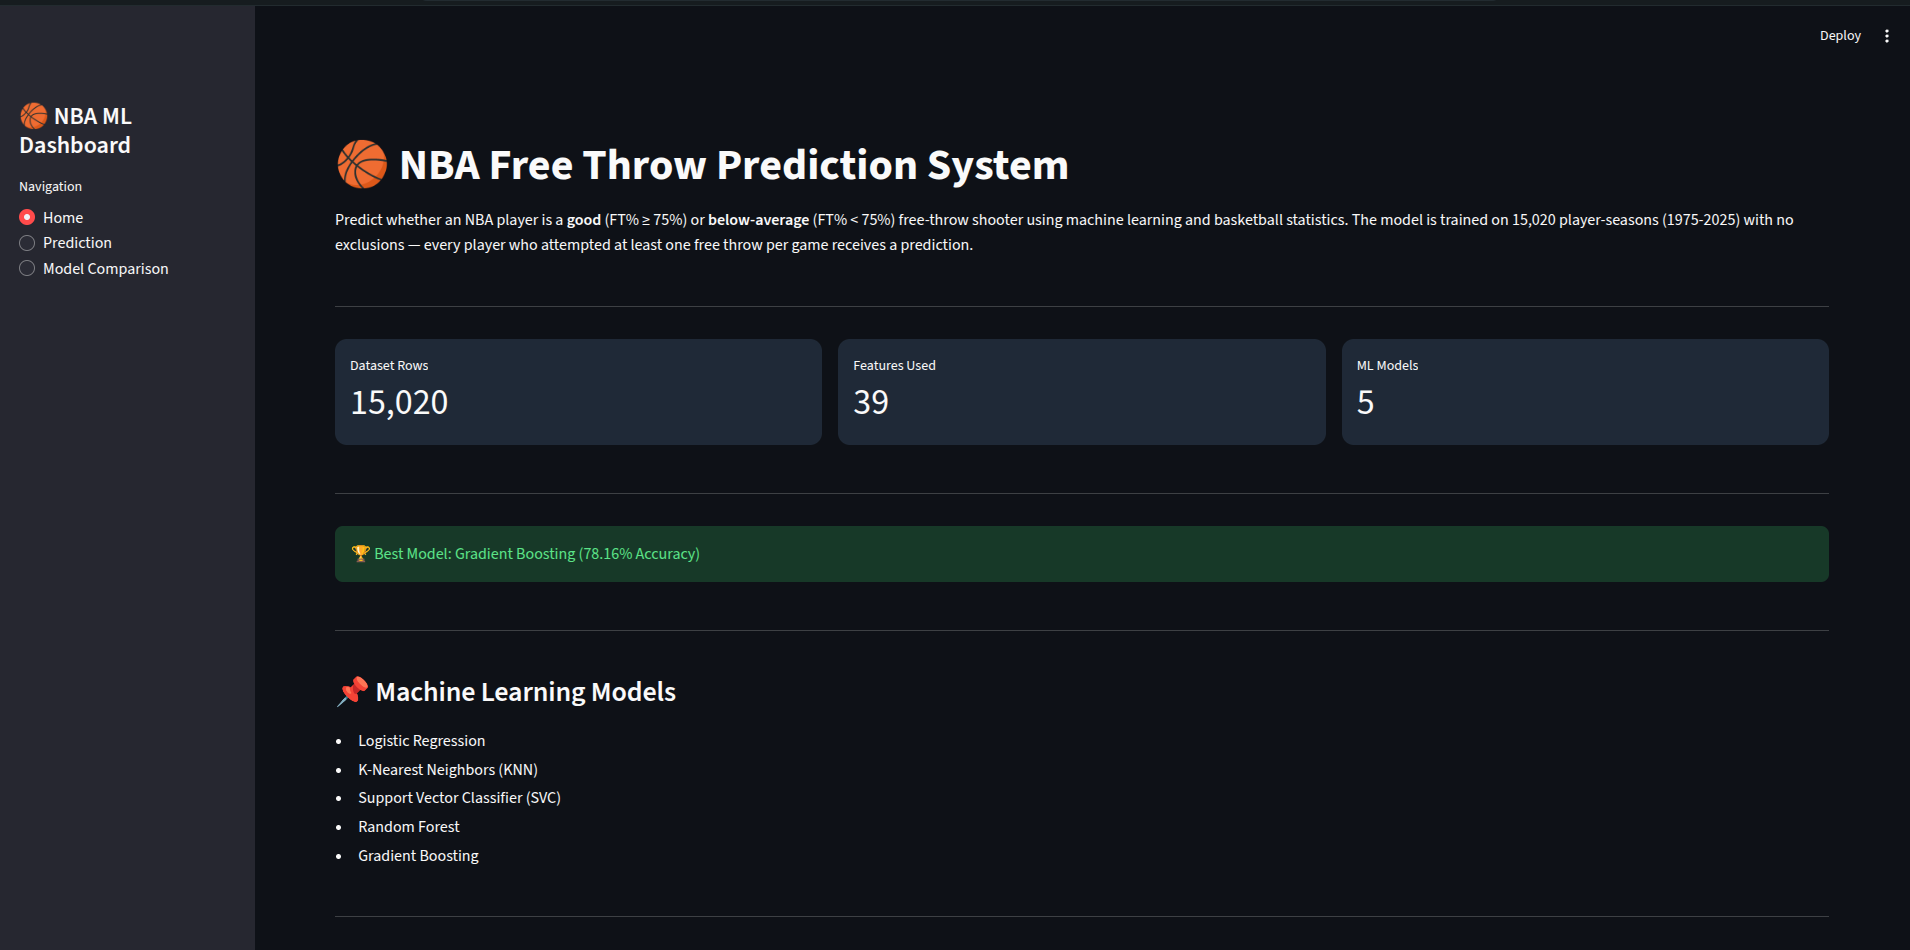
\includegraphics[width=0.48\textwidth]{streamlit_home.png}
\caption{Streamlit application --- Home page.}
\label{fig:home}
\end{figure}

\begin{figure}[H]
\centering
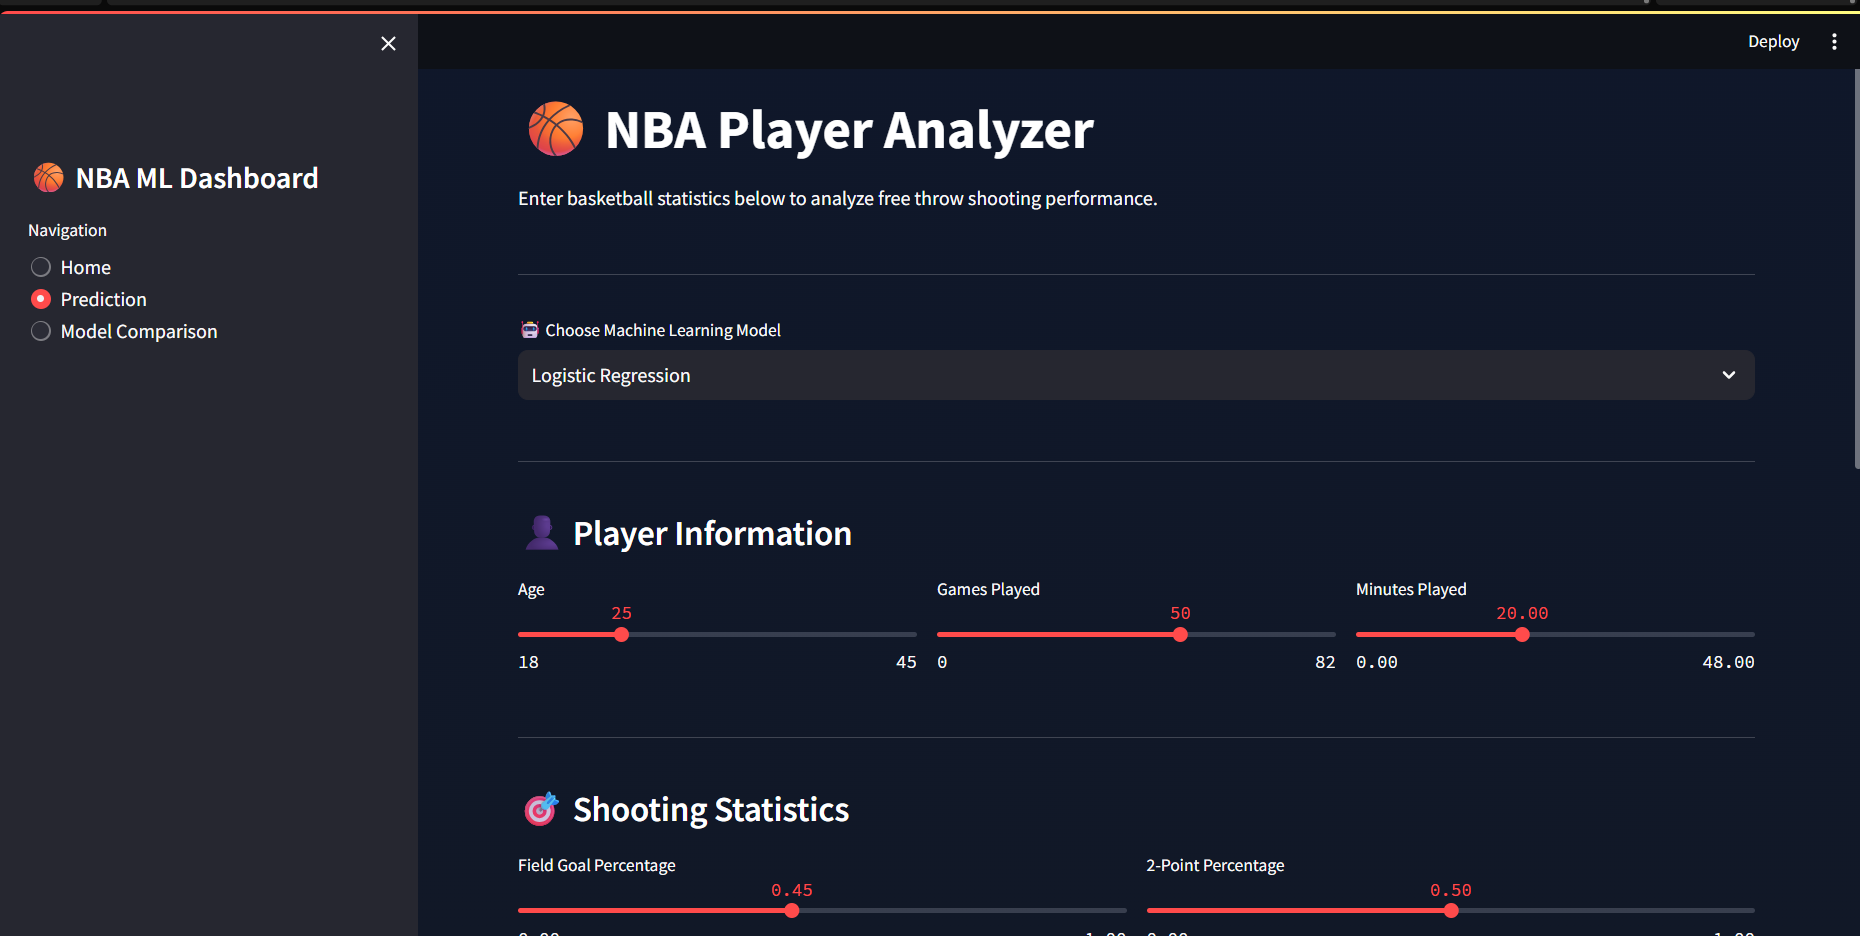
\includegraphics[width=0.48\textwidth]{streamlit_prediction.png}
\caption{Streamlit application --- Prediction page.}
\label{fig:prediction}
\end{figure}

% =========================================================
% LIMITATIONS
% =========================================================

\section{Limitations}

Several limitations were identified during the project:

\begin{itemize}
\item Season-average statistics hide game-to-game consistency: two players with the same FT\% may differ greatly in reliability.
\item Psychological and situational factors --- clutch pressure, fatigue, crowd effects --- are not represented in box-score data.
\item Injury history and changes in shooting mechanics across a career are not captured.
\item Coaching, training regimens, and practice habits are unavailable.
\item NBA playstyles and rules changed substantially between 1975 and 2025, introducing era-related variation into the features.
\item The external bio merge could not match roughly 490 player-seasons by name; these were filled with median values.
\end{itemize}

% =========================================================
% CONCLUSION
% =========================================================

\section{Conclusion}

This project presented a complete machine learning pipeline for classifying NBA player-seasons as good or below-average free-throw shooters. An original dataset of 26{,}292 player-season records was assembled by web scraping two Basketball Reference sources and integrating them. The data underwent careful preprocessing, with particular emphasis on preventing data leakage by excluding all current-season free-throw quantities from the feature set, yielding 15{,}020 modeling rows described by 39 features.

Five classification algorithms were trained with default-configuration estimators and compared on an identical test set. Gradient Boosting achieved the best test accuracy at 78.06\%, closely followed by SVC and Random Forest. The 71--78\% range across all models is an honest reflection of the difficulty of the task once every player --- including the genuinely uncertain cases --- must be classified. Finally, the system was deployed as an interactive Streamlit web application that delivers real-time predictions and model comparison. Overall, the project demonstrates both the value and the realistic limits of machine learning in sports analytics, and the importance of leakage-aware experimental design.

% =========================================================
% FUTURE WORK
% =========================================================

\section{Future Work}

Future improvements may include incorporating advanced and tracking-based NBA statistics, modeling game-level rather than season-average data to capture consistency, adding more external data sources such as college or international shooting records, experimenting with deep learning architectures, integrating a live NBA data API for automatic updates, and deploying the dashboard to a public cloud platform.

% =========================================================
% REFERENCES
% =========================================================

\begin{thebibliography}{00}

\bibitem{b1}
Basketball Reference,
Available:
\url{https://www.basketball-reference.com}

\bibitem{b2}
Basketball Reference Leagues,
Available:
\url{https://www.basketball-reference.com/leagues/}

\bibitem{b3}
F. Pedregosa et al.,
``Scikit-learn: Machine Learning in Python,''
\textit{Journal of Machine Learning Research}, vol. 12, pp. 2825--2830, 2011.
Available: \url{https://scikit-learn.org}

\bibitem{b4}
Streamlit Documentation,
Available:
\url{https://streamlit.io}

\bibitem{b5}
A. G\'eron,
\textit{Hands-On Machine Learning with Scikit-Learn, Keras, and TensorFlow},
3rd ed., O'Reilly Media, 2022.

\bibitem{b6}
T. Hastie, R. Tibshirani, and J. Friedman,
\textit{The Elements of Statistical Learning},
2nd ed., Springer, 2009.

\bibitem{b7}
L. Breiman,
``Random Forests,''
\textit{Machine Learning}, vol. 45, no. 1, pp. 5--32, 2001.

\bibitem{b8}
J. H. Friedman,
``Greedy Function Approximation: A Gradient Boosting Machine,''
\textit{Annals of Statistics}, vol. 29, no. 5, pp. 1189--1232, 2001.

\end{thebibliography}

\end{document}
